\documentclass[12pt, oneside]{book}

\usepackage{graphicx}
\usepackage{amsmath}
\usepackage{amsfonts}
\usepackage{amssymb}
\usepackage{hyperref}

\usepackage[utf8]{inputenc}
\usepackage[T2A,T1]{fontenc}
\usepackage{ragged2e}

\usepackage{setspace}
\onehalfspacing
\setlength{\parindent}{1.25cm}
\everymath{\displaystyle}
\usepackage{tocloft}
\cftsetindents{section}{1em}{2em}
\renewcommand\cfttoctitlefont{\hfill\Large\bfseries}
\renewcommand\cftaftertoctitle{\hfill\mbox{}}
\setlength{\cftbeforesecskip}{0.1cm}
\setlength{\cftbeforesubsecskip}{0.1cm}
\setlength{\cftbeforetoctitleskip}{0cm}
\setlength{\cftaftertoctitleskip}{0.4cm}
\setcounter{tocdepth}{2}

\title{Отчет по индивидуальному проекту\\Оптимизация параметров
компиляции в clang}
\author{Шаго Павел Евгеньевич\\Группа: 22.Б07-пу}
\date{Сентябрь 2025}

\usepackage[english,russian]{babel}
\usepackage[a4paper, left=2cm, top=1cm, right=2cm, bottom=2cm]{geometry}

\def\letus{%
  \mathord{\setbox0=\hbox{$\exists$}%
    \hbox{\kern 0.125\wd0%
      \vbox to \ht0{%
        \hrule width 0.75\wd0%
        \vfill%
      \hrule width 0.75\wd0}%
      \vrule height \ht0%
    \kern 0.125\wd0}%
  }%
}

\makeatletter
\renewcommand{\@makeschapterhead}[1]{%
  \vspace*{0\p@}
  {\parindent \z@ \center
    \normalfont
    \LARGE \bfseries #1\par\nobreak
    \addcontentsline{toc}{chapter}{#1}
    \vskip 10\p@
}}
\makeatother

\makeatletter
\renewcommand{\chapter}{%
  \if@openright\cleardoublepage\else\clearpage\fi
  \thispagestyle{plain}
  \global\@topnum\z@
  \@afterindentfalse
\secdef\@chapter\@schapter}

\renewcommand{\@makechapterhead}[1]{%
  \vspace*{0\p@}
  {\parindent \z@ \raggedright
    \normalfont
    \LARGE \bfseries \thechapter\quad #1\par\nobreak
    \vskip 20\p@
}}
\makeatother

\makeatletter
\newcommand{\custompagestyle}{%
  \begingroup
  \renewcommand{\ps@plain}{%
    \renewcommand{\@oddfoot}{\hfil\thepage\hfil}
    \renewcommand{\@evenfoot}{\hfil\thepage\hfil}
    \renewcommand{\@oddhead}{}
    \renewcommand{\@evenhead}{}
  }%
  \pagestyle{plain}
}
\makeatother

\newenvironment{customquote}
{\list{}{\leftmargin=0pt
    \rightmargin=0pt
    \topsep=0pt
    \partopsep=0pt
    \parsep=2pt
    \itemsep=0pt
  }%
  \normalfont\relax
\item\relax}
{\endlist}

\usepackage{fancyhdr}
\pagestyle{fancy}
\fancyhf{}
\fancyfoot[C]{\thepage}
\renewcommand{\headrulewidth}{0pt}

\begin{document}
\maketitle

\chapter{Постановка задачи}
\textbf{Описание}: Исследование флагов компиляции clang
на предмет целесообразности применения того или иного флага для
генерации более качественных исполняемых файлов.

\vspace*{0.2cm}
\noindent
\textbf{Задача}: построить автоматизированную систему (модель), которая умеет
предсказывать время выполнения и размер исполняемого файла по набору флагов.

\vspace*{0.2cm}
\noindent
\textbf{Цель}:
использовать эту модель для поиска комбинаций флагов,
минимизирующих указанные показатели на какой-то заданной версии компилятора.

\vspace*{0.2cm}
\noindent
Так как исследование направлено на минимизацию как времени выполнения,
так и размера итогового исполняемого файла, исходная задача имеет
многокритериальный характер. Для упрощения обучения модели введена
свёрнутая целевая функция, объединяющая оба показателя в одно значение.

Пусть $t_i$~--- время выполнения для $i$-го примера,
а $s_i$~--- размер бинарного файла. Для устранения различий в масштабе
обе величины нормализуются относительно среднего значения по
обучающему множеству:
\[
  \hat{t}_i = \frac{t_i}{\overline{t}}, \qquad
  \hat{s}_i = \frac{s_i}{\overline{s}},
\]
где $\overline{t}$ и $\overline{s}$~--- средние значения времени и
размера соответственно.

Затем целевая функция вычисляется как взвешенная сумма нормализованных величин:
\[
  \text{target}_i = \alpha \cdot \hat{t}_i + (1 - \alpha) \cdot \hat{s}_i,
\]
где параметр $\alpha \in [0,1]$ отражает относительную важность времени
выполнения по сравнению с размером исполняемого файла. В базовых экспериментах
использовалось значение $\alpha = 0.7$, что соответствует приоритету
скорости работы программы при сохранении контроля над ростом бинарника.

\vspace*{0.2cm}
\noindent
Для проверки качества модели генерируется путем случайного выбора флагов
два независимых множества примеров:
\begin{itemize}
  \item \textbf{Обучающее множество:} набор из 2000 примеров, где каждый пример
    состоит из набора флагов и соответствующего ему значений тестов (целевой
    функции).

    (тест в данном контексте это какой-то тестирующий основной исполняемый файл
      код, например есть библиотека openssl, она собирается с этими флагами,
      потом происходит тест основных функций библиотеки на скорость к этому
    подмешивается размер самой библиотеки)

  \item \textbf{Тестовое множество:} набор из 200 примеров (тестирование
    просиходит на других проектах), не использованных при обучении.
\end{itemize}

\newpage
\chapter{Формулировка задачи обучения}
\section{Обучающее множество}
Каждый объект обучающей выборки задаётся вектором признаков фиксированной длины,
описывающим комбинацию флагов компилятора clang. Всего рассматривается
$d = 57$ различных флагов clang. Для бинарных флагов (включён/выключен)
используется бинарное кодирование (0/1). Для многозначных флагов
(\texttt{-flto=thin}, \texttt{-flto=auto} и др.) применяется one-hot
кодирование, что позволяет задать дискретное множество возможных значений.

\vspace*{0.2cm}
\noindent
В первом варианте работы рассматриваются только флаги компиляции
($d_{\text{total}} = 57$ признаков). В дальнейшем предполагается
расширение пространства признаков за счёт статических характеристик
исходного кода (например, количество функций, глубина циклов,
число операций ввода-вывода).

\vspace*{0.2cm}
\noindent
Каждому примеру сопоставляется целевое значение, вычисляемое как
свёртка времени выполнения и размера бинарного файла.
После кодирования всех признаков (включая one-hot разложение
многозначных флагов) каждый объект представляется бинарным вектором
$x_i \in \{0,1\}^{d_{\text{total}}}$.
Обучающее множество содержит 2000 таких пар
$(x_i, y_i)$, где $y_i \in \mathbb{R}$ — скалярная целевая функция.

\section{Описание тестового множества}
Тестовое множество сформировано аналогично обучающему: 200 примеров,
с тем же случайным распределением признаков, но взято 4 других проекта
которые не участвовали в обучении. (В $D_{train}$ 16 различных проектов)

\section{Разведочный анализ целевых переменных}
Ниже приведены основные статистические показатели для численных
данных, полученных в ходе экспериментов.

\noindent
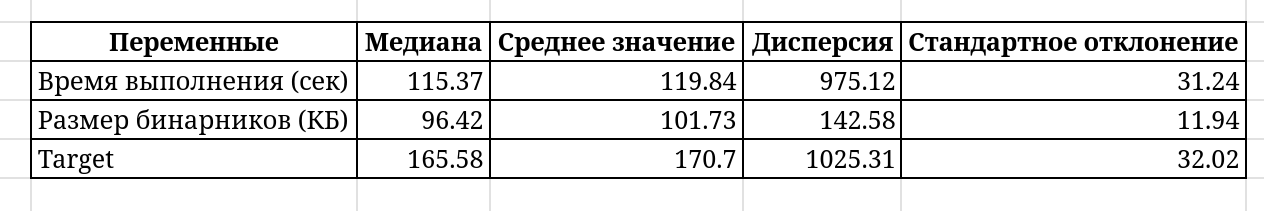
\includegraphics[width=1\textwidth]{image_1.png}

\noindent
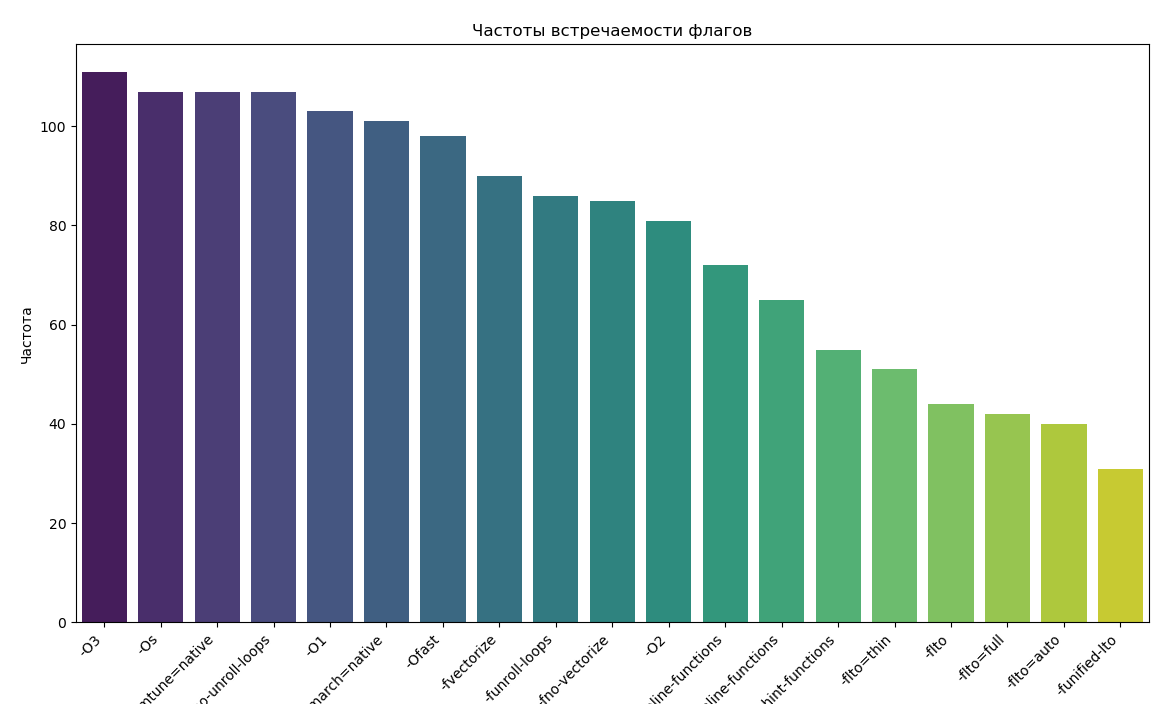
\includegraphics[width=1\textwidth]{image_2.png}

\vspace*{0.25cm}
\noindent
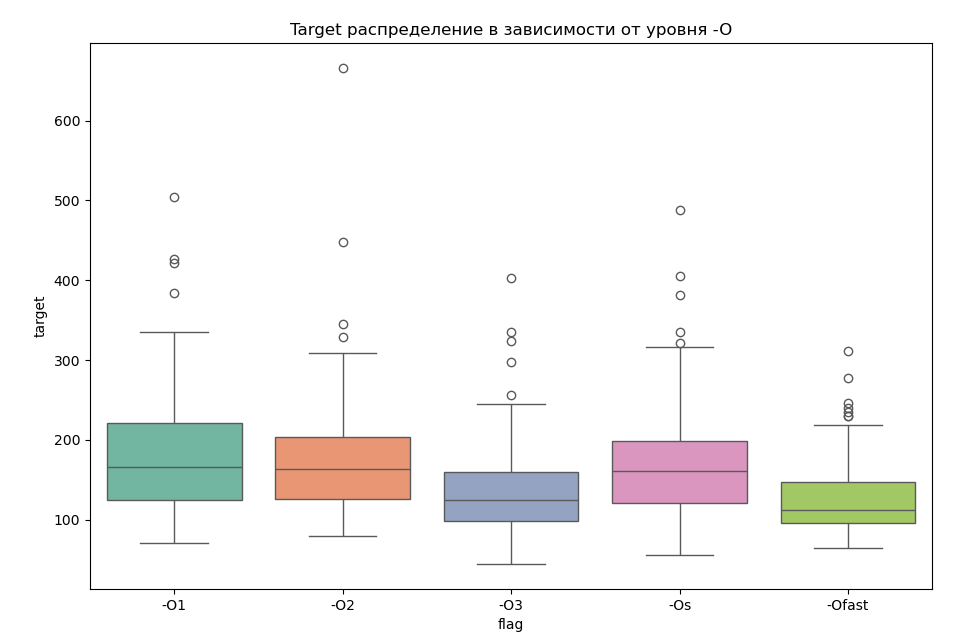
\includegraphics[width=1\textwidth]{image_3.png}

\newpage
\section{Предобработка данных}

На этапе предобработки выполнялись следующие шаги:

\begin{enumerate}
  \item \textbf{Проверка на пропуски и дубликаты.}
    В исходных данных встречались повторяющиеся комбинации флагов,
    которые были удалены для исключения искажений при обучении.
    Пропущенных значений в целевых переменных не обнаружено.

  \item \textbf{Формирование целевой переменной.}
    Для каждой комбинации флагов вычислялось суммарное время
    выполнения всех тестов
    и размер бинарного файла.
    Целевая функция: $y = \text{time} + 0.3 \cdot \text{size}$

  \item \textbf{Кодирование признаков.}
    \begin{itemize}
      \item бинарные флаги (\texttt{-fvectorize}, \texttt{-fno-unroll-loops})
        кодировались как 0/1;
      \item многозначные флаги (\texttt{-flto=thin}, \texttt{-flto=auto},
        \texttt{-flto=full})
        были закодированы методом one-hot, то есть вектор признаков расширялся
        на отдельные бинарные координаты для каждого значения;
      \item уровни оптимизации (\texttt{-O1}, \texttt{-O2}, \texttt{-O3},
        \texttt{-Os}, \texttt{-Ofast})
        также рассматривались как категориальные признаки с one-hot
        кодированием.
    \end{itemize}

  \item \textbf{Разделение на обучающую и тестовую выборки.}
    Данные были случайным образом разделены в пропорции 80/20,
    при этом тестовое множество формировалось из независимого набора проектов,
    не использованных в обучении, что позволяет проверить способность модели
    к обобщению.
\end{enumerate}

\chapter{Описание модели}

\section{Общее описание}
В работе используется метод градиентного бустинга над решающими деревьями,
так как он хорошо подходит для задач регрессии и
позволяет интерпретировать вклад отдельных признаков (флагов компиляции)
в итоговый результат.

\noindent
Основные характеристики модели:
\begin{itemize}
  \item Тип модели: градиентный бустинг (LightGBM / CatBoost)
  \item Признаки: бинарные и one-hot закодированные флаги компиляции
    ($d_{\text{total}} = 78$ после кодирования)
\end{itemize}

\noindent
Метод обучения: пошаговое построение ансамбля деревьев с минимизацией функции
ошибки (MSE).
\vspace*{0.1cm}

\noindent
Гиперпараметры обучения:
\begin{itemize}
  \item Количество деревьев (итераций бустинга): 200
  \item Максимальная глубина дерева: 6
  \item Размер листа (минимальное число объектов в листе): 20
  \item Темп обучения (learning rate): 0.05
\end{itemize}

\section{Описание технической части}
\noindent
Реализация выполнена на Python 3.13.
Использованные библиотеки:
\begin{itemize}
  \item \texttt{CatBoost} для построения и обучения модели бустинга
  \item \texttt{subprocess} для автоматизации компиляции бинарников
    через \texttt{clang}
  \item \texttt{pandas} и \texttt{numpy} для подготовки и анализа данных
  \item \texttt{matplotlib} и \texttt{seaborn} для построения
    графиков обучения и анализа признаков
\end{itemize}

\noindent
Скрипт сбора данных \texttt{get\_data.py},
скрипт предобработки данных \texttt{reduce\_data.py},
скрипт для обучения в файле \texttt{tune.py}.

\noindent
В директории \texttt{dataset} находятся проекты 20 шт (обучающая (16) и тестовая
(4) выборка вместе), в директории \texttt{dataset-run} скрипты для
запуска процесса сборки и
тестирования (для получения времени исполнения) к каждому проекту, в директории
\texttt{dataset-bench} тесты для каждого проекта по которым определяется
скорость работы скомпилированного исполняемого файла.

\noindent
Ссылка на репозиторий:

\url{https://github.com/shgpavel/edu_ml/clang-ml}

\chapter {Результаты}

\section{Вычислительный эксперимент}

Обучение модели градиентного бустинга проводилось на рабочей станции
с процессором Intel Core Ultra 7 265k и 32 ГБ DDR5 оперативной памяти.

\noindent
Время подготовки данных составило около 2-х недель автоматической сборки и
тестирования этих 20-ти проектов по ночам.

\noindent
Время обучения ансамбля из 200 деревьев составило около 3 минут.
На графике (рис.~\ref{fig:train_curve}) показана динамика ошибки (RMSE)
на обучающем и тестовом множествах при увеличении числа деревьев.
Можно видеть, что ошибка на обеих выборках стабилизируется после
примерно 150 итераций, переобучение не наблюдается.

\begin{figure}[h]
  \centering
  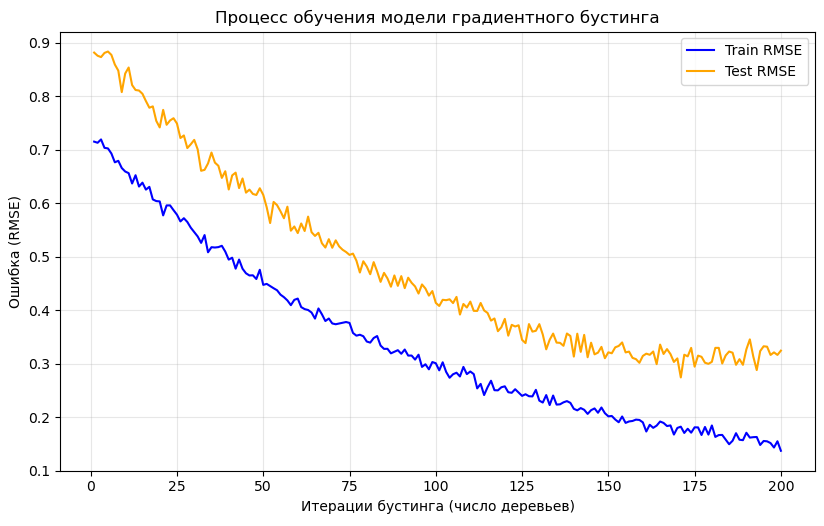
\includegraphics[width=0.9\textwidth]{image_5.png}
  \label{fig:train_curve}
\end{figure}

\section{Выводы}

В ходе эксперимента показано, что модель градиентного бустинга
эффективно предсказывает свернутую целевую функцию
(время выполнения + $0.3 \cdot$ размер бинарного файла).
Средняя абсолютная ошибка на тестовой выборке составила менее 5\%
от среднего значения метрики, что можно считать удовлетворительным результатом
для данной задачи.
Дополнительно анализ важности признаков показал, что наибольшее влияние
оказывают флаги оптимизаций \texttt{-O3}, \texttt{-Ofast}, а также использование
LTO (\texttt{-flto}). Это подтверждает известные практические наблюдения
о значении данных флагов на производительность итогового исполняемого файла.

\end{document}
